\documentclass[a4paper,oneside,12pt]{report}
% Package yang diperlukan
\usepackage{fontspec}       % Font sistem untuk XeLaTeX/LuaLaTeX
\usepackage{setspace}       % Pengaturan jarak antarbaris
\usepackage{graphicx}      % Untuk memasukkan gambar
\usepackage{titling}       % Untuk kustomisasi halaman judul
\usepackage{geometry}      % Untuk mengatur margin halaman
\usepackage{listings}      % Untuk menampilkan blok kode
\usepackage{xcolor}        % Untuk menggunakan warna
\usepackage{float}         % Untuk kontrol penempatan float (seperti gambar)
\usepackage{xurl}          % Untuk pemutusan tautan URL yang lebih baik
\usepackage{hyperref}      % Untuk membuat hyperlink (URL, referensi)
\usepackage{indentfirst}   % Untuk memberi indentasi pada paragraf pertama setiap seksi
\usepackage{url}           % Untuk format URL
\usepackage{fancyhdr}      % Untuk kustomisasi header dan footer
\usepackage{tocloft}       % Untuk kustomisasi Daftar Isi
\usepackage{bookmark}      % Untuk manajemen bookmark PDF yang lebih baik
\usepackage{amsmath}       % Untuk rumus matematika
\usepackage{amssymb}       % Untuk simbol matematika
\usepackage{booktabs}      % Untuk tabel yang lebih rapi
\usepackage{caption}
\usepackage{subcaption}    % Untuk tata letak gambar berdampingan
\usepackage{tabularx}      % Untuk tabel dengan lebar otomatis sesuai margin
\usepackage{array}         % Untuk kontrol kolom tabel
\usepackage{enumitem}      % Untuk kontrol kerapatan daftar
\usepackage[none]{hyphenat} % Nonaktifkan seluruh pemotongan kata bertanda hubung
\usepackage{microtype}     % Tipografi halus dan protrusion antislop

% Font dan spasi standar laporan praktikum
\setmainfont{Times New Roman}
\onehalfspacing

%======================================================================
% PENGATURAN GEOMETRI HALAMAN
%======================================================================
\geometry{left=3cm, right=2.5cm, top=2cm, bottom=2.5cm}
\sloppy
\tolerance=10000
\emergencystretch=3em
\hfuzz=1.5pt
\hbadness=10000
\hyphenpenalty=10000
\exhyphenpenalty=10000
\righthyphenmin=62
\lefthyphenmin=62

%======================================================================
% PENGATURAN WARNA UNTUK BLOK KODE
%======================================================================
\definecolor{codegreen}{rgb}{0,0.6,0}
\definecolor{codegray}{rgb}{0.5,0.5,0.5}
\definecolor{codepurple}{rgb}{0.58,0,0.82}
\definecolor{backcolour}{rgb}{0.95,0.95,0.92}
\definecolor{darkblue}{rgb}{0,0,0.6}

%======================================================================
% PENGATURAN BLOK KODE (LISTINGS)
%======================================================================
\lstdefinestyle{commonstyle}{
    backgroundcolor=\color{backcolour},
    breakatwhitespace=false,
    breaklines=true,
    captionpos=b,
    keepspaces=true,
    numbers=left,
    numbersep=5pt,
    showspaces=false,
    showstringspaces=false,
    showtabs=false,
    tabsize=2,
    frame=single,
    basicstyle=\ttfamily\scriptsize,
    numberstyle=\tiny\color{codegray},
    columns=flexible,
    postbreak=\mbox{\textcolor{red}{$\hookrightarrow$}\space},
    breakindent=0pt,
    breakautoindent=false
}
\lstdefinestyle{pythonstyle}{
    style=commonstyle,
    language=Python,
    commentstyle=\color{codegreen},
    keywordstyle=\color{darkblue},
    stringstyle=\color{codepurple},
    emph={import,from,class,def,for,while,if,else,elif,try,except,finally},
    emphstyle=\color{darkblue}
}

\lstdefinestyle{bashstyle}{
    style=commonstyle,
    language=bash,
    numbers=none,
    commentstyle=\color{codegreen},
    keywordstyle=\color{black},
    stringstyle=\color{codepurple}
}

%======================================================================
% PENGATURAN LAIN-LAIN
%======================================================================
\newcommand{\customfbox}[1]{%
  \setlength{\fboxsep}{0pt}%
  \setlength{\fboxrule}{0.5pt}%
  \fcolorbox{black}{white}{#1}%
}
\renewcommand{\figurename}{Gambar}
\renewcommand{\thefigure}{\arabic{figure}}
\renewcommand{\tablename}{Tabel}
\renewcommand{\thetable}{\arabic{table}}
\renewcommand{\theequation}{\arabic{equation}}
\renewcommand{\lstlistingname}{Listing}
\AtBeginDocument{\renewcommand{\thelstlisting}{\arabic{lstlisting}}}
\counterwithout{figure}{chapter}
\counterwithout{table}{chapter}
\counterwithout{equation}{chapter}
\hypersetup{
    colorlinks=true,
    linkcolor=black,
    filecolor=black,
    urlcolor=black,
    citecolor=black,
    pdftitle={Laporan Praktikum Penambangan Data Pertemuan 10},
    pdfpagemode=FullScreen,
    breaklinks=true
}
\pagestyle{fancy}
\fancyhf{}
\fancyfoot[C]{\thepage}
\renewcommand{\headrulewidth}{0pt}
\fancypagestyle{plain}{
    \fancyhf{}
    \fancyfoot[C]{\thepage}
    \renewcommand{\headrulewidth}{0pt}
}
\renewcommand{\contentsname}{Daftar Isi}
\renewcommand{\bibname}{Daftar Pustaka}
\renewcommand{\thechapter}{}
\renewcommand{\chaptername}{}
\renewcommand{\thesection}{\arabic{chapter}.\arabic{section}}
\renewcommand{\thesubsection}{\thesection.\arabic{subsection}}
\setcounter{secnumdepth}{3}
\setcounter{tocdepth}{3}
\renewcommand{\cftchapdotsep}{\cftdotsep}
\renewcommand{\cftchapleader}{\cftdotfill{\cftchapdotsep}}
\setlength{\cftchapindent}{0em}
\setlength{\cftsecindent}{2em}
\setlength{\cftsubsecindent}{4em}
\setlength{\cftchapnumwidth}{0em}
\setlength{\cftsecnumwidth}{2.5em}
\setlength{\cftsubsecnumwidth}{3.2em}
\setlength{\cftbeforechapskip}{4pt}
\setlength{\cftbeforesecskip}{1.5pt}
\setlength{\cftbeforesubsecskip}{0.5pt}
\renewcommand{\cftchappresnum}{}
\renewcommand{\cftchapaftersnum}{}
\newcommand{\tocboldsection}[1]{%
  \protect\renewcommand{\protect\cftchapfont}{\protect\bfseries}%
  #1%
  \protect\renewcommand{\protect\cftchapfont}{}%
}

%======================================================================
% AWAL DOKUMEN
%======================================================================
\begin{document}

% Halaman Judul
\newgeometry{left=3cm, right=2.5cm, top=2.5cm, bottom=3cm}
\begin{titlingpage}
	\begin{spacing}{1}
		\begin{center}
			\vspace*{0.2cm}
			{\large \textbf{\MakeUppercase{Laporan Praktikum}}} \\[0.4cm]
			{\large \textbf{\MakeUppercase{Praktikum Penambangan Data}}} \\[0.4cm]
			{\large \textbf{\MakeUppercase{Pertemuan 10}}} \\[0.4cm]
			{\large \textbf{\MakeUppercase{Model Deployment (Flask)}}} \\[1.5cm]

			
\includegraphics[height=7cm]{images/UGM.png} \\[0.7cm]

			{\normalsize \textbf{Disusun oleh:}} \\[0.4cm]
			\begin{tabular}{@{}l l @{}}
				\textbf{Nama}           & : Hafidz Rizqullah Prasetya        \\
				\textbf{NIM}            & : 24/535493/SV/24243               \\
				\textbf{Kelas}          & : PL5A1                            \\
				\textbf{Dosen Pengampu} & : Dr. Imam Fahrurrozi, S.T., M.Cs.
			\end{tabular} \\[1.2cm]

			{\normalsize \textbf{PROGRAM STUDI D-IV}} \\[0.2cm]
			{\normalsize \textbf{TEKNOLOGI REKAYASA PERANGKAT LUNAK}} \\[0.2cm]
			{\normalsize \textbf{DEPARTEMEN TEKNIK ELEKTRO DAN INFORMATIKA}} \\[0.2cm]
			{\normalsize \textbf{SEKOLAH VOKASI}} \\[0.2cm]
			{\normalsize \textbf{UNIVERSITAS GADJAH MADA}} \\[0.2cm]
			{\normalsize \textbf{YOGYAKARTA}} \\[0.2cm]
			{\normalsize \textbf{2026}} \\[1.2cm]
		\end{center}
	\end{spacing}
\end{titlingpage}
\restoregeometry

\thispagestyle{empty}
\clearpage
\stepcounter{page}
\thispagestyle{empty}

% --- Daftar Isi ---
\addcontentsline{toc}{chapter}{Daftar Isi}
\begin{spacing}{0.92}
	\tableofcontents
\end{spacing}
\clearpage

% Mengatur penomoran halaman menjadi arab dan mulai dari 3
\pagenumbering{arabic}
\setcounter{page}{3}

\chapter[Tujuan Praktikum]{Tujuan Praktikum}
Berdasarkan Modul Pertemuan 10 Praktikum Penambangan Data, tujuan praktikum ini adalah:
\begin{enumerate}[noitemsep, topsep=4pt, parsep=2pt]
	\item Memahami konsep dasar \textit{model deployment} dalam siklus hidup \textit{data mining} (\textit{ML lifecycle}).
	\item Melakukan \textit{serialization} (penyimpanan) dan \textit{deserialization} (pemuatan kembali) model \textit{machine learning} dengan pustaka \texttt{joblib} atau \texttt{pickle}.
	\item Membangun layanan web (\textit{web service}) sederhana dengan \textit{micro-framework} Flask.
	\item Mengintegrasikan model \textit{machine learning} ke antarmuka web dan API sehingga pengguna dapat mengirim data baru dan menerima hasil prediksi.
\end{enumerate}

\clearpage

\chapter{Dasar Teori}

\section{Model Deployment dalam Siklus Hidup Machine Learning}
Pengembangan model \textit{machine learning} berjalan sebagai siklus: perumusan masalah, pengumpulan data, penyiapan data, eksplorasi, rekayasa fitur, pelatihan, evaluasi, lalu \textit{deployment} dan pemantauan \cite{han2022}. Sampai Pertemuan 9, pekerjaan saya berhenti di tahap evaluasi. Model hanya hidup di dalam \textit{notebook}, sehingga orang lain tidak bisa memakainya tanpa menjalankan ulang seluruh kode pelatihan.

\textit{Deployment} adalah tahap yang membuat model bisa dipakai oleh pengguna atau sistem lain. Modul menyebut tiga skema: model yang ditanam langsung di aplikasi (\textit{embedded}), prediksi berkala untuk banyak data sekaligus (\textit{batch prediction}), dan arsitektur \textit{client-server}. Praktikum ini memakai skema \textit{client-server}. Model disimpan di server, sedangkan klien (peramban atau program lain) mengirim data lewat protokol HTTP dan menerima hasil prediksi sebagai halaman HTML atau JSON.

\section{Alur Client-Server dan Metode HTTP}
Pada skema \textit{client-server}, satu permintaan prediksi melewati lima langkah. Klien membuka alamat (\textit{endpoint}) yang disediakan server, lalu mengirim nilai fitur lewat form web atau badan permintaan JSON. Server mengurai dan memvalidasi masukan itu, kemudian menyusunnya menjadi bentuk yang diminta model. Model yang sudah dimuat ke memori menghitung prediksi, dan server mengirim hasilnya kembali ke klien.

Dua metode HTTP yang dipakai di praktikum ini adalah GET untuk meminta halaman dan POST untuk mengirim data. Server membalas dengan kode status, misalnya 200 untuk permintaan yang berhasil, 400 untuk masukan yang salah, 404 untuk alamat yang tidak ada, dan 500 untuk galat di sisi server. Gaya arsitektur yang memperlakukan setiap alamat sebagai sumber daya dan memakai metode HTTP apa adanya dikenal sebagai REST \cite{fielding2000}.

\section{Flask}
Flask adalah \textit{micro web framework} berbahasa Python. Intinya hanya mengurus perutean (\textit{routing}), objek permintaan dan balasan, serta \textit{template} HTML lewat Jinja. Basis data dan validasi form tidak disertakan dan boleh ditambahkan sendiri bila perlu \cite{flask-quickstart}. Sifat ini cocok untuk membungkus model, karena kode pelatihan dan kode server sama-sama Python sehingga objek model dapat langsung dipanggil di dalam fungsi \textit{route}.

Sebuah \textit{route} didefinisikan dengan dekorator \texttt{@app.route}. Nilai form dibaca dari \texttt{request.form}, badan JSON dibaca dengan \texttt{request.get\_json()}, halaman dikembalikan dengan \texttt{render\_template}, dan balasan JSON dibuat dengan \texttt{jsonify}. Perintah \texttt{app.run()} menjalankan server pengembangan bawaan Werkzeug. Dokumentasi Flask menyatakan server ini hanya untuk pengembangan; untuk produksi aplikasi dijalankan di belakang server WSGI seperti Gunicorn \cite{flask-deploy}.

\section{Serialisasi Model}
Model yang selesai dilatih hanya ada di memori dan hilang ketika proses Python berakhir. \textit{Serialization} mengubah objek model menjadi deretan \textit{byte} yang disimpan sebagai berkas, dan \textit{deserialization} memuat berkas itu kembali menjadi objek yang siap dipakai tanpa pelatihan ulang. Python menyediakan modul \texttt{pickle} untuk keperluan ini, sedangkan \texttt{joblib} memakai mekanisme yang sama tetapi lebih efisien untuk objek berisi \textit{array} NumPy besar \cite{joblib-persistence}. Fungsinya adalah \texttt{joblib.dump(model, berkas)} dan \texttt{joblib.load(berkas)}.

Ada dua hal yang perlu diingat. Pertama, memuat berkas \texttt{pickle} dapat menjalankan kode apa pun yang tersimpan di dalamnya, jadi berkas model hanya boleh dimuat dari sumber yang dipercaya \cite{python-pickle}. Kedua, dokumentasi scikit-learn tidak menjamin model yang disimpan dengan satu versi dapat dimuat dengan versi lain, sehingga versi pustaka saat pelatihan sebaiknya dicatat bersama modelnya \cite{sklearn-persistence}.

\section{Decision Tree}
Percobaan modul memakai \texttt{DecisionTreeClassifier}. Pohon keputusan membagi data secara berulang dengan satu pertanyaan pada satu fitur di setiap simpul. Scikit-learn mengimplementasikan algoritma CART \cite{breiman1984, sklearn2011} dan secara bawaan memilih pembagian yang paling menurunkan ketidakmurnian Gini:
\begin{equation}
	G = 1 - \sum_{k=1}^{K} p_k^2
\end{equation}
dengan $p_k$ proporsi sampel kelas $k$ pada simpul tersebut. Nilai $G = 0$ berarti simpul hanya berisi satu kelas.

\section{Support Vector Machine dan Kalibrasi Probabilitas}
Model terbaik pada bagian tugas adalah \textit{Support Vector Machine} (SVM) dengan kernel \textit{radial basis function} (RBF). SVM mencari bidang pemisah dengan margin terlebar di antara dua kelas \cite{cortes1995}. Kernel RBF mengukur kemiripan dua sampel dengan
\begin{equation}
	K(x, x') = \exp\left(-\gamma \lVert x - x' \rVert^2\right)
\end{equation}
sehingga batas keputusan boleh berbentuk tidak linier. Karena kernel ini bergantung pada jarak, setiap fitur distandarkan lebih dahulu dengan $z = (x - \mu) / \sigma$ agar fitur berskala besar seperti usia tidak mendominasi.

Keluaran asli SVM adalah jarak bertanda ke bidang pemisah, bukan probabilitas. Untuk mendapat peluang, jarak itu dipetakan dengan fungsi sigmoid yang parameternya dicari lewat validasi silang (metode Platt) \cite{platt1999}. Di scikit-learn, langkah ini dikerjakan oleh \texttt{CalibratedClassifierCV} \cite{sklearn-calibration}.

Performa klasifikasi diukur dengan \textit{accuracy}, \textit{precision}, \textit{recall}, dan \textit{F1-score}:
\begin{align}
	\text{Precision} & = \frac{TP}{TP + FP}, \qquad \text{Recall} = \frac{TP}{TP + FN} \\
	\text{F1-Score}  & = \frac{2 \cdot \text{Precision} \cdot \text{Recall}}{\text{Precision} + \text{Recall}}
\end{align}

\clearpage

\chapter{Alat dan Bahan}

\section{Perangkat Keras}
\begin{enumerate}[noitemsep, topsep=2pt, parsep=1pt]
	\item Laptop dengan prosesor 12 \textit{thread} dan RAM 14 GB.
	\item Koneksi internet untuk mengunduh berkas proyek modul.
\end{enumerate}

\section{Perangkat Lunak}
\begin{enumerate}[noitemsep, topsep=2pt, parsep=1pt]
	\item Sistem operasi Linux Mint 22.3 64-bit.
	\item Python 3.12.3 di dalam \textit{virtual environment}.
	\item Terminal dengan \textit{shell} zsh untuk menjalankan skrip dan server.
	\item Peramban Google Chrome 156 untuk menguji antarmuka web.
	\item cURL 8.5.0 untuk menguji \textit{endpoint} API.
	\item Pustaka Python:
	      \begin{itemize}[noitemsep, topsep=1pt, parsep=0.5pt]
		      \item \texttt{flask} 3.1.3: layanan web.
		      \item \texttt{scikit-learn} 1.9.1: pelatihan dan evaluasi model.
		      \item \texttt{pandas} 3.0.5 dan \texttt{numpy} 2.5.3: pengolahan data tabular.
		      \item \texttt{joblib} 1.6.0: serialisasi model.
	      \end{itemize}
\end{enumerate}

\section{Dataset}
\begin{enumerate}[noitemsep, topsep=2pt, parsep=1pt]
	\item Dataset HCV (\texttt{hcvdat0.csv}) dari berkas proyek modul \cite{uci-hcv}, berisi 615 baris hasil uji laboratorium donor darah dan pasien hepatitis C dengan 12 fitur.
	\item Dataset \textit{Early Stage Diabetes Risk Prediction} \cite{uci-diabetes, islam2020} yang dipakai proyek kelompok saya (Kelompok 3, GlucoSense), berisi 520 baris kuesioner pasien dengan 16 fitur.
\end{enumerate}

\clearpage

\chapter[\texorpdfstring{\tocboldsection{Hasil dan Pembahasan}}{Hasil dan Pembahasan}]{Hasil dan Pembahasan}

Seluruh percobaan saya jalankan langsung di laptop lewat terminal dan peramban, tanpa \textit{notebook}, sesuai catatan modul bahwa server Flask tidak disarankan dijalankan di dalam Jupyter. Semua tangkapan layar pada bab ini diambil dari terminal dan peramban di laptop tersebut. Kode lengkap tersedia di repositori berikut:

\begin{center}
	\href{https://github.com/hafidzrizqullahprasetya/PPD/tree/main/pertemuan-10}{\textcolor{blue}{\url{https://github.com/hafidzrizqullahprasetya/PPD/tree/main/pertemuan-10}}} \cite{repo-kode}
\end{center}

\section{Percobaan Modul: Deployment Model Klasifikasi Penyakit Hati}

\subsection{Persiapan Direktori dan Dataset}
Berkas proyek saya unduh dari tautan Google Drive pada modul. Arsipnya berukuran sekitar 300 MB karena juga memuat contoh model citra, jadi saya hanya mengambil dua folder yang diminta modul, yaitu \texttt{flask/create\_model/tabular} dan \texttt{flask/web/tabular\_v2}.

\begin{figure}[H]
	\centering
	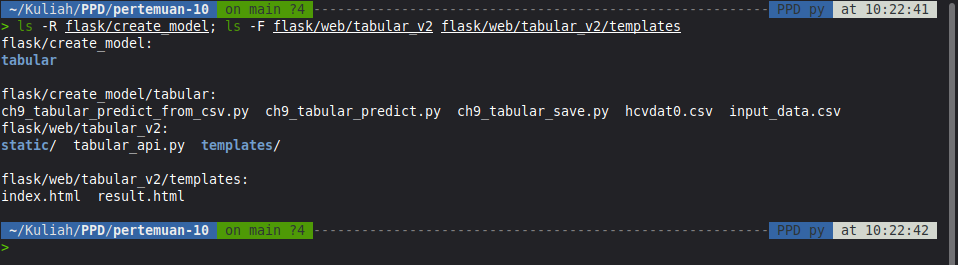
\includegraphics[width=0.9\textwidth]{images/ss-01-struktur-folder-modul.png}
	\caption{Isi folder pelatihan model dan folder aplikasi web dari berkas proyek modul.}
	\label{fig:ss-struktur-modul}
\end{figure}

Folder \texttt{tabular} berisi dataset \texttt{hcvdat0.csv} beserta tiga skrip: satu untuk melatih dan menyimpan model, dua untuk mencoba prediksi. Folder \texttt{tabular\_v2} berisi skrip server \texttt{tabular\_api.py}, folder \texttt{templates} untuk halaman HTML, dan folder \texttt{static} untuk berkas CSS dan JavaScript.

Pustaka saya pasang dengan perintah dari modul. Flask belum ada di \textit{virtual environment} saya, sedangkan empat pustaka lain sudah terpasang sejak pertemuan sebelumnya.

\begin{figure}[H]
	\centering
	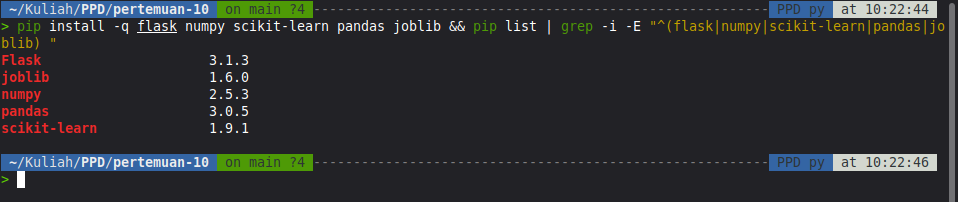
\includegraphics[width=0.9\textwidth]{images/ss-02-instal-pustaka.png}
	\caption{Pemasangan pustaka dan versi yang terpasang.}
	\label{fig:ss-instal}
\end{figure}

\subsection{Pelatihan dan Serialisasi Model}
Skrip pelatihan pada modul bernama \texttt{ch9\_tabular\_save.py}. Skrip ini membaca dataset, membuang baris yang memiliki nilai kosong, memisahkan fitur dari label \texttt{Category}, mengubah label teks menjadi angka 0 sampai 3, mengodekan kolom \texttt{Sex} dengan \texttt{LabelEncoder}, lalu melatih \texttt{DecisionTreeClassifier} dan menyimpannya dengan \texttt{joblib.dump}.

\begin{lstlisting}[style=pythonstyle,caption={Inti skrip pelatihan dan serialisasi model (\texttt{ch9\_tabular\_save.py}).}]
def dt(X, y):
    model = DecisionTreeClassifier(random_state=0)
    model = model.fit(X, y)
    filename = 'dt_model.model'
    joblib.dump(model, filename)

if __name__ == '__main__':
    df_ori = pd.read_csv('hcvdat0.csv')
    df_ori = df_ori.dropna()
    df_X = df_ori.drop(['Unnamed: 0','Category'],axis=1)
    df_y = df_ori['Category']
    df_y=df_y.replace('0=Blood Donor',0)
    df_y=df_y.replace('0s=suspect Blood Donor',0)
    df_y=df_y.replace('1=Hepatitis',1)
    df_y=df_y.replace('2=Fibrosis',2)
    df_y=df_y.replace('3=Cirrhosis',3)
    df_y = df_y.astype(int)       # baris tambahan saya

    df_X_numb = df_X.drop(['Sex'], axis=1)
    le = preprocessing.LabelEncoder()
    df_X['Sex'] = le.fit_transform(df_X['Sex'])
    df_X_new = pd.concat([df_X['Sex'], df_X_numb], axis=1)
    dt(df_X_new, df_y)
\end{lstlisting}

Saat pertama kali saya jalankan apa adanya, skrip berhenti dengan galat seperti pada Gambar~\ref{fig:ss-galat-label}.

\begin{figure}[H]
	\centering
	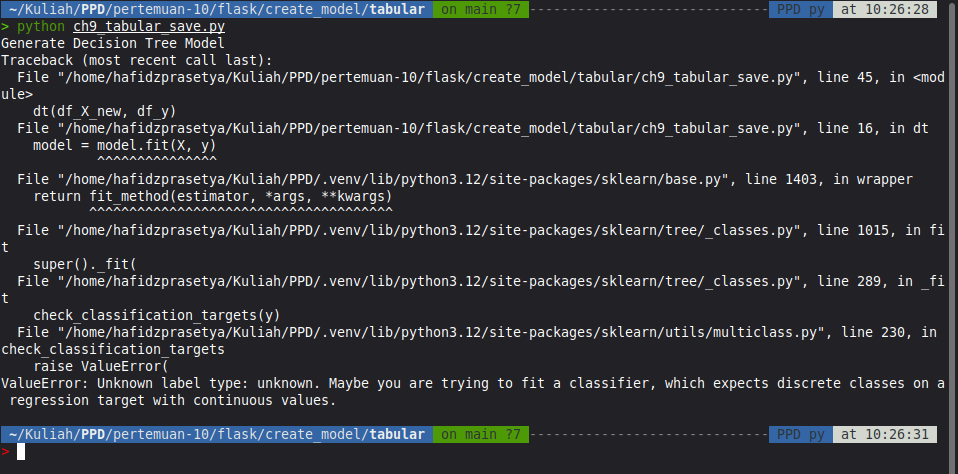
\includegraphics[width=0.9\textwidth]{images/ss-03-galat-label-kelas.png}
	\caption{Galat \texttt{Unknown label type} saat skrip modul dijalankan tanpa perubahan.}
	\label{fig:ss-galat-label}
\end{figure}

Penyebabnya ada di kolom label. Skrip modul ditulis tahun 2020, sedangkan saya memakai pandas 3.0.5. Di versi ini, kolom \texttt{Category} yang semula berisi teks tetap bertipe \texttt{object} setelah \texttt{replace}, walaupun isinya sudah angka 0 sampai 3. Scikit-learn tidak mengenali tipe itu sebagai label kelas sehingga menolak melatih model. Saya menambahkan satu baris \texttt{df\_y = df\_y.astype(int)} setelah proses pelabelan ulang, dan pelatihan berhasil.

\begin{figure}[H]
	\centering
	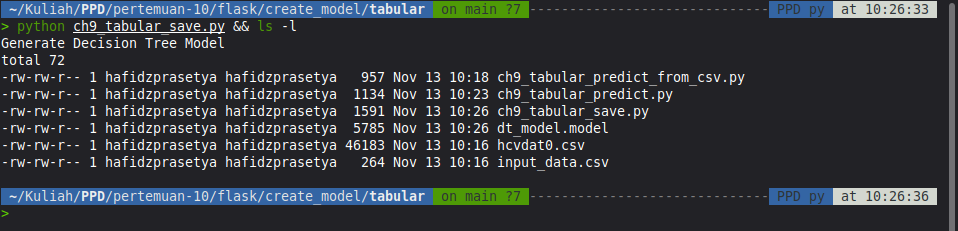
\includegraphics[width=0.9\textwidth]{images/ss-04-latih-simpan-model.png}
	\caption{Skrip pelatihan berhasil dan berkas \texttt{dt\_model.model} terbentuk.}
	\label{fig:ss-latih-dt}
\end{figure}

Berkas \texttt{dt\_model.model} berukuran 5.785 \textit{byte}. Dari 615 baris data, 589 baris tersisa setelah baris kosong dibuang. Pohon yang terbentuk memiliki kedalaman 6 dengan 22 daun. Ada dua catatan tentang model ini. Skrip modul melatih pohon pada seluruh data tanpa data uji, jadi tidak ada angka akurasi yang bisa saya laporkan, dan model ini memang hanya dipakai sebagai bahan latihan \textit{deployment}. Selain itu kelasnya sangat timpang: 533 baris berlabel 0 (donor darah), sedangkan hepatitis 20 baris, fibrosis 12 baris, dan sirosis 24 baris.

\subsection{Uji Deserialisasi dari Skrip}
Sebelum masuk ke Flask, saya mencoba memuat kembali model dengan dua skrip prediksi dari modul. Skrip pertama membuat satu baris data baru di dalam kode, skrip kedua membaca empat baris dari \texttt{input\_data.csv}.

\begin{figure}[H]
	\centering
	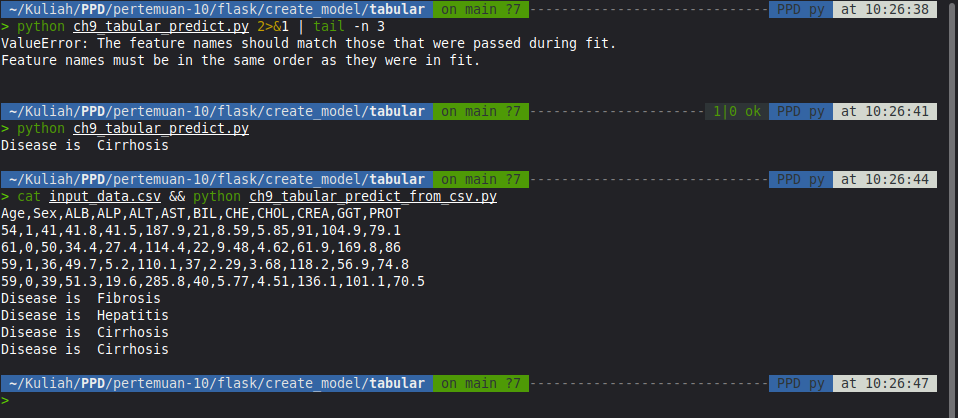
\includegraphics[width=0.9\textwidth]{images/ss-05-prediksi-skrip.png}
	\caption{Galat urutan fitur pada skrip prediksi asli, lalu hasil prediksi setelah urutan kolom diperbaiki.}
	\label{fig:ss-prediksi-skrip}
\end{figure}

Skrip prediksi asli juga gagal, kali ini dengan pesan \texttt{Feature names must be in the same order as they were in fit}. Model dilatih dengan urutan kolom \texttt{Sex}, \texttt{Age}, \texttt{ALB}, dan seterusnya, karena skrip pelatihan menaruh kolom \texttt{Sex} paling depan lewat \texttt{pd.concat}. Skrip prediksi menyusun kolom dengan urutan \texttt{Age}, \texttt{Sex}, \texttt{ALB}. Scikit-learn versi sekarang menyimpan nama fitur saat \texttt{fit} dan menolak data dengan urutan berbeda. Menurut saya pemeriksaan ini sangat membantu. Tanpa itu, nilai usia akan terbaca sebagai jenis kelamin dan model tetap mengeluarkan prediksi yang salah tanpa pesan apa pun.

Perbaikannya saya lakukan di sisi data masukan. Pada skrip pertama urutan kolom saya ubah menjadi \texttt{Sex} dahulu. Pada skrip kedua saya menambahkan \texttt{df\_input = df\_input[loaded\_model.feature\_names\_in\_]} supaya urutan kolom CSV mengikuti urutan yang tersimpan di model. Setelah itu skrip pertama memprediksi \textit{Cirrhosis}, dan empat baris CSV diprediksi \textit{Fibrosis}, \textit{Hepatitis}, \textit{Cirrhosis}, dan \textit{Cirrhosis}. Model yang dimuat dari berkas bekerja tanpa pelatihan ulang, jadi proses serialisasi dan deserialisasi berhasil.

\subsection{Web Service Flask dan Endpoint Prediksi}
Kode server pada modul ada di berkas \texttt{tabular\_api.py} dan memiliki dua \textit{route}. \textit{Route} \texttt{/tabular/} menampilkan form \texttt{index.html}. \textit{Route} \texttt{/tabular/result/} menerima kiriman form dengan metode POST, memuat model, menjalankan prediksi, lalu menampilkan \texttt{result.html}.

Versi \texttt{tabular\_api.py} di dalam arsip unduhan masih menyusun kolom dengan urutan \texttt{Age} lalu \texttt{Sex}, sehingga terkena galat yang sama dengan skrip prediksi. Kode pada Gambar 10.4.10 modul sudah versi yang diperbaiki, jadi saya menyesuaikan berkas saya dengan kode di modul tersebut. Versi ini menambahkan dua fungsi bantu. Fungsi \texttt{\_to\_float} mengubah teks dari form menjadi bilangan, dan \texttt{\_encode\_sex} menerima isian seperti \texttt{m}, \texttt{male}, atau \texttt{1} lalu mengubahnya menjadi 1.

\noindent\begin{minipage}{\linewidth}
\begin{lstlisting}[style=pythonstyle,caption={Potongan \textit{endpoint} prediksi pada \texttt{tabular\_api.py}.}]
app = Flask(__name__)

@app.route("/tabular/")
def index():
    return render_template('index.html')

@app.route('/tabular/result/', methods=["POST"])
def prediction_result():
    age = request.form.get('age')
    sex = request.form.get('sex')
    # ... sepuluh fitur lain dibaca dengan cara yang sama
    loaded_model = joblib.load('dt_model.model')
    sex_enc = _encode_sex(sex)
    columns_order = ['Sex', 'Age', 'ALB', 'ALP', 'ALT', 'AST',
                     'BIL', 'CHE', 'CHOL', 'CREA', 'GGT', 'PROT']
    df_input = pd.DataFrame(columns=columns_order)
    df_input.loc[0] = [sex_enc, _to_float(age), _to_float(alb), ...]
    result = loaded_model.predict(df_input)
    # ... angka 0 sampai 3 dipetakan ke nama penyakit
    return render_template('result.html', age=age, sex=sex, ...,
                           status=decision)
\end{lstlisting}
\end{minipage}

Berkas \texttt{dt\_model.model} kemudian saya salin ke folder \texttt{tabular\_v2}, karena server mencari berkas model di folder tempat ia dijalankan.

\begin{figure}[H]
	\centering
	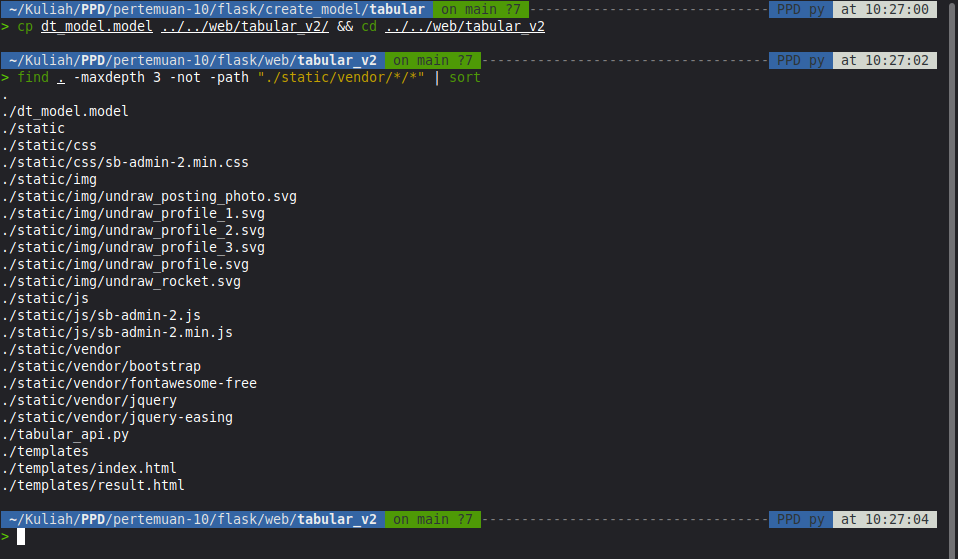
\includegraphics[width=0.82\textwidth]{images/ss-06-struktur-proyek-flask.png}
	\caption{Penyalinan model dan struktur proyek aplikasi Flask.}
	\label{fig:ss-struktur-flask}
\end{figure}

Struktur ini mengikuti konvensi Flask. Halaman HTML harus berada di folder \texttt{templates} agar ditemukan oleh \texttt{render\_template}, dan berkas CSS, JavaScript, serta ikon berada di folder \texttt{static} yang otomatis dilayani pada alamat \texttt{/static/}.

\subsection{Menjalankan Server dan Pengujian}
Server saya jalankan dengan \texttt{python tabular\_api.py}, lalu saya buka \texttt{http://127.0.0.1:5000/tabular/} di peramban.

\begin{figure}[H]
	\centering
	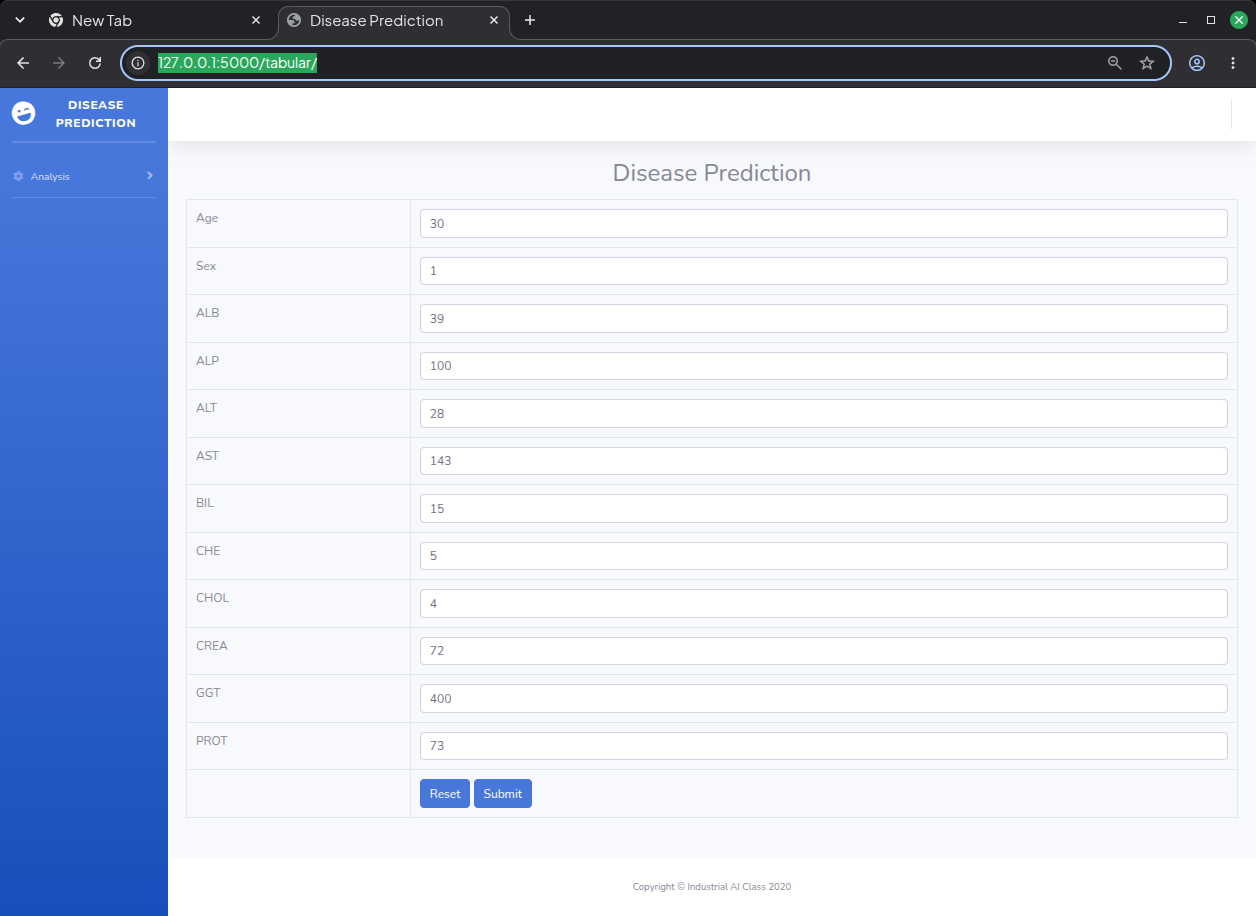
\includegraphics[width=0.9\textwidth]{images/ss-08-form-tabular.png}
	\caption{Form masukan data klinis pada \textit{endpoint} \texttt{/tabular/}.}
	\label{fig:ss-form-tabular}
\end{figure}

Form menampilkan 12 kolom isian dengan nilai bawaan dari \textit{template}. Nilai bawaan itu saya kirim dengan menekan tombol \textit{Submit}.

\begin{figure}[H]
	\centering
	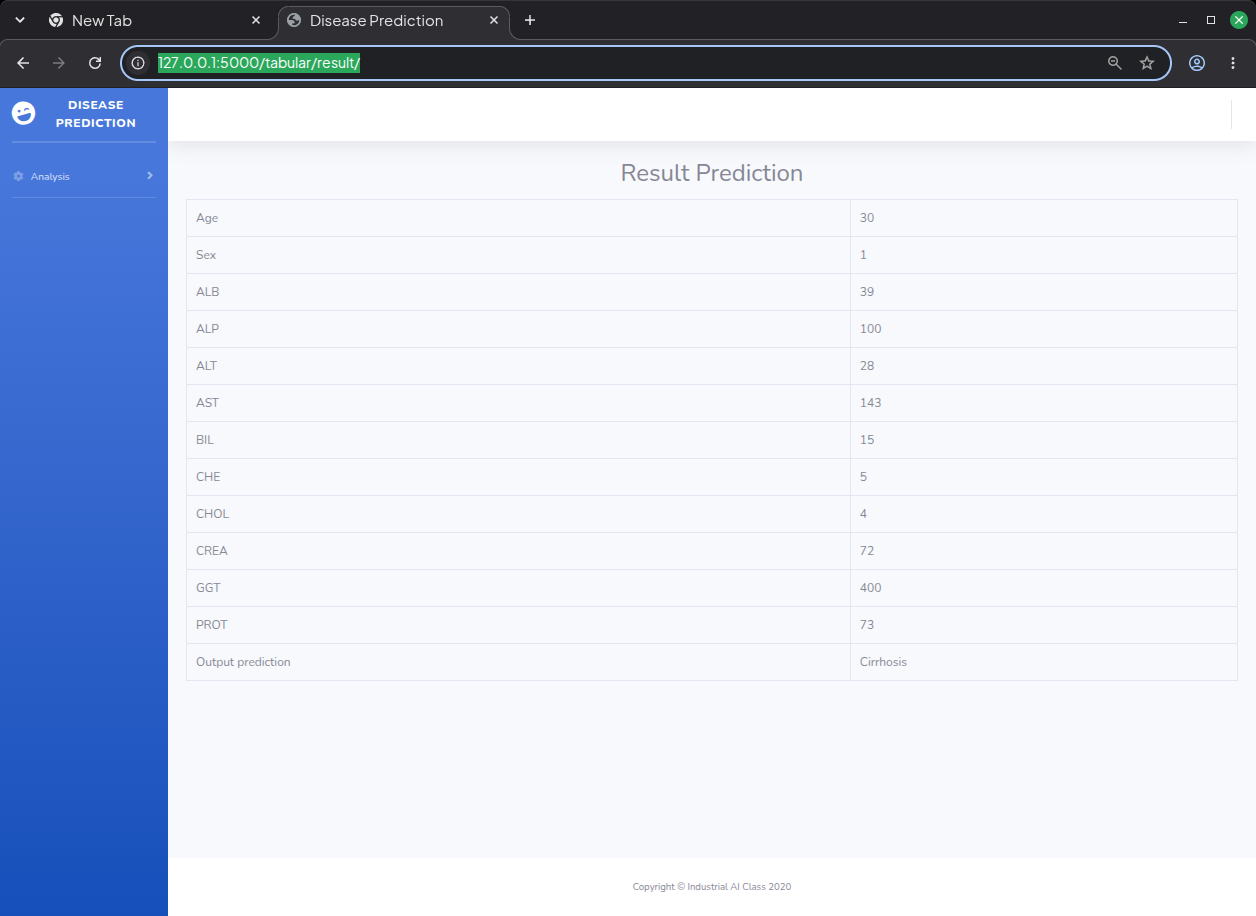
\includegraphics[width=0.9\textwidth]{images/ss-09-hasil-tabular.png}
	\caption{Halaman hasil prediksi pada \textit{endpoint} \texttt{/tabular/result/}.}
	\label{fig:ss-hasil-tabular}
\end{figure}

Halaman hasil menampilkan kembali 12 nilai yang dikirim dan prediksi \textit{Cirrhosis} pada baris \textit{Output prediction}. Nilai AST 143 dan GGT 400 pada isian ini memang jauh di atas kebanyakan donor sehat di dataset, jadi prediksi sirosis masuk akal.

\begin{figure}[H]
	\centering
	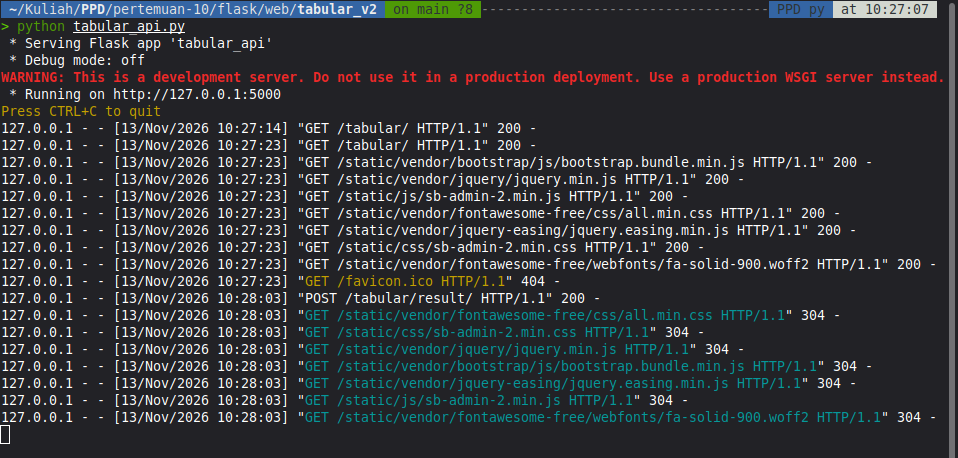
\includegraphics[width=0.9\textwidth]{images/ss-07-jalankan-flask-modul.png}
	\caption{Log server Flask modul selama pengujian.}
	\label{fig:ss-log-modul}
\end{figure}

Log server pada Gambar~\ref{fig:ss-log-modul} memperlihatkan alur \textit{client-server} yang dijelaskan di dasar teori. Permintaan \texttt{GET /tabular/} dibalas 200, lalu peramban meminta berkas CSS dan JavaScript dari \texttt{/static/}. Saat tombol \textit{Submit} ditekan, muncul baris \texttt{POST /tabular/result/} dengan status 200. Kode 304 pada permintaan berikutnya berarti peramban memakai salinan berkas statis yang sudah tersimpan, dan 404 untuk \texttt{favicon.ico} muncul karena aplikasi ini tidak punya ikon. Baris peringatan berwarna merah mengingatkan bahwa server bawaan ini hanya untuk pengembangan.

Dari percobaan modul ini saya mencatat dua kelemahan pada aplikasinya. Model dimuat ulang dengan \texttt{joblib.load} di setiap permintaan, dan form menerima teks bebas tanpa validasi. Kolom \textit{Sex} misalnya harus diisi angka 1 atau 0, tanpa keterangan mana yang laki-laki. Keduanya saya perbaiki pada aplikasi tugas.

\clearpage

\section{Tugas dan Analisis: Aplikasi Web GlucoSense}
Tugas modul meminta dataset proyek kelompok dipakai untuk melatih model, model terbaiknya diserialisasi, lalu dibuatkan antarmuka web dengan Flask. Proyek Kelompok 3 bernama GlucoSense, yaitu deteksi dini risiko diabetes dari gejala klinis awal. Dataset berisi usia, jenis kelamin, dan 14 gejala berjawaban ya atau tidak, misalnya sering buang air kecil (\textit{polyuria}) dan sering haus (\textit{polydipsia}), dengan label \textit{Positive} atau \textit{Negative}. Bagian saya di kelompok adalah pemodelan dan \textit{backend} prediksi, jadi tugas ini sekaligus menjadi rancangan awal untuk bagian tersebut.

\subsection{Pelatihan dan Pemilihan Model}
Skrip \texttt{train\_model.py} mengikuti prapemrosesan yang sudah disepakati kelompok: baris duplikat dihapus, jawaban \textit{Yes/No} diubah menjadi 1/0, \textit{Male/Female} menjadi 1/0, dan data dibagi 70\% latih dan 30\% uji secara terstratifikasi. Bedanya dengan \textit{notebook} kelompok, penskalaan dan model saya gabungkan dalam satu objek \texttt{Pipeline}.

\noindent\begin{minipage}{\linewidth}
\begin{lstlisting}[style=pythonstyle,caption={Pencarian \textit{hyperparameter} dan pemilihan model pada \texttt{train\_model.py}.}]
cv = StratifiedKFold(n_splits=5, shuffle=True, random_state=SEED)
hasil, terbaik = [], None
for nama, (estimator, grid) in kandidat_model().items():
    pipa = Pipeline([('scaler', StandardScaler()), ('model', estimator)])
    cari = GridSearchCV(pipa, grid, cv=cv, scoring='f1', n_jobs=-1)
    cari.fit(X_train, y_train)
    ...
    if terbaik is None or cari.best_score_ > terbaik[1].best_score_:
        terbaik = (nama, cari)

nama, cari = terbaik
model = cari.best_estimator_
joblib.dump(model, MODEL_DIR / 'glucosense_model.joblib')
\end{lstlisting}
\end{minipage}

Ada tiga kandidat, yaitu \textit{Logistic Regression}, \textit{Random Forest}, dan SVM berkernel RBF. Masing-masing dicari \textit{hyperparameter} terbaiknya dengan \texttt{GridSearchCV} dan validasi silang 5 lipatan pada data latih. Model dipilih dari rata-rata F1 validasi silang, bukan dari skor data uji. Untuk SVM saya membungkusnya dengan \texttt{CalibratedClassifierCV}, karena parameter \texttt{probability=True} pada \texttt{SVC} sudah berstatus \textit{deprecated} di scikit-learn 1.9 dan aplikasi web membutuhkan nilai peluang.

\begin{figure}[H]
	\centering
	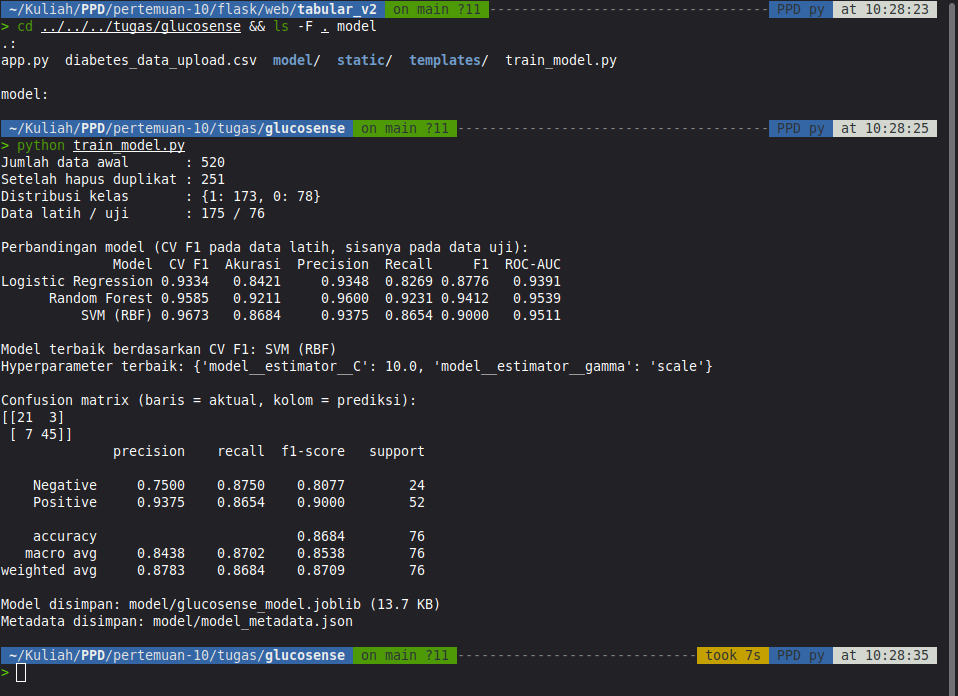
\includegraphics[width=0.88\textwidth]{images/ss-10-latih-model-diabetes.png}
	\caption{Keluaran \texttt{train\_model.py}: perbandingan model, model terpilih, dan evaluasinya.}
	\label{fig:ss-latih-diabetes}
\end{figure}

Dari 520 baris, 269 baris ternyata duplikat sehingga tersisa 251 pasien, terdiri atas 173 positif dan 78 negatif. Data latih berisi 175 baris dan data uji 76 baris. Tabel~\ref{tab:komparasi-model} merangkum hasil ketiga kandidat.

\begin{table}[H]
	\centering
	\caption{Perbandingan tiga kandidat model pada dataset diabetes.}
	\label{tab:komparasi-model}
	\small
	\begin{tabular}{|l|c|c|c|c|c|c|}
		\hline
		\textbf{Model}               & \textbf{F1 CV}  & \textbf{Akurasi} & \textbf{Precision} & \textbf{Recall} & \textbf{F1}     & \textbf{ROC-AUC} \\
		\hline
		\textit{Logistic Regression} & 0,9334          & 0,8421           & 0,9348             & 0,8269          & 0,8776          & 0,9391           \\
		\hline
		\textit{Random Forest}       & 0,9585          & \textbf{0,9211}  & \textbf{0,9600}    & \textbf{0,9231} & \textbf{0,9412} & \textbf{0,9539}  \\
		\hline
		SVM (RBF)                    & \textbf{0,9673} & 0,8684           & 0,9375             & 0,8654          & 0,9000          & 0,9511           \\
		\hline
	\end{tabular}
\end{table}

SVM memiliki F1 validasi silang tertinggi (0,9673) dengan $C = 10$ dan $\gamma$ bawaan, sehingga model inilah yang disimpan. Hasil di data uji ternyata berbeda: \textit{Random Forest} lebih baik dengan akurasi 0,9211, sedangkan SVM 0,8684. Saya tetap menyimpan SVM. Kalau model dipilih karena angka ujinya paling tinggi, data uji ikut dipakai untuk mengambil keputusan dan angkanya tidak lagi mewakili data yang belum pernah dilihat. Selisih kedua model juga kecil dibanding ukuran datanya. Di data uji selisih itu setara 4 dari 76 pasien, dan selisih F1 validasi silang hanya 0,0088. Dengan data sesedikit ini saya belum bisa menyimpulkan salah satu model benar-benar lebih unggul. Pilihan final untuk proyek kelompok masih perlu dibahas bersama anggota lain, misalnya dengan validasi silang berulang.

Pada \textit{confusion matrix} SVM, 45 dari 52 pasien positif terdeteksi dan 7 pasien positif diprediksi negatif (\textit{false negative}). Sebaliknya, 3 dari 24 pasien negatif diprediksi positif. Untuk alat skrining, 7 kasus yang lolos itu lebih merugikan daripada 3 alarm palsu, karena pasien yang sebenarnya berisiko bisa merasa aman. \textit{Recall} 0,8654 ini menjadi kelemahan utama model saat ini.

\subsection{Berkas Model dan Metadata}
\begin{figure}[H]
	\centering
	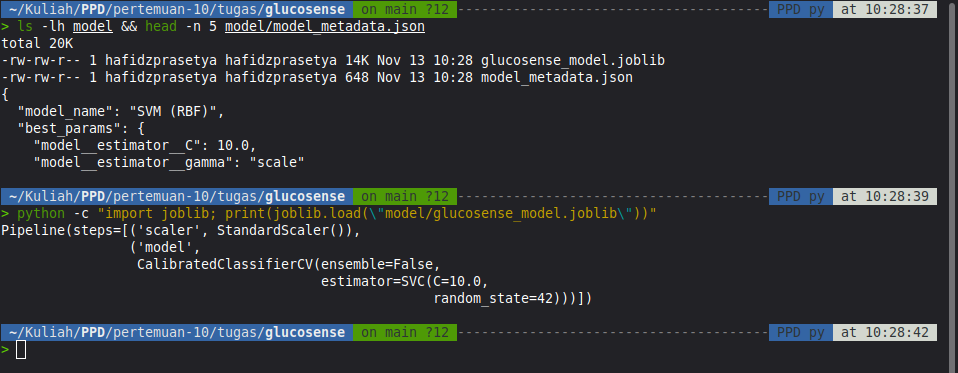
\includegraphics[width=0.9\textwidth]{images/ss-11-berkas-model.png}
	\caption{Berkas hasil serialisasi dan isi \texttt{Pipeline} saat dimuat kembali.}
	\label{fig:ss-berkas-model}
\end{figure}

Pelatihan menghasilkan dua berkas, yaitu model \texttt{glucosense\_model.joblib} sebesar 14 KB dan \texttt{model\_metadata.json}. Saat dimuat kembali dengan \texttt{joblib.load}, objeknya adalah \texttt{Pipeline} berisi \texttt{StandardScaler} dan SVM terkalibrasi. Pada proyek kelompok, \textit{scaler} dan model disimpan sebagai dua berkas terpisah, sehingga aplikasi web harus ingat memanggil keduanya dengan urutan yang benar. Dengan satu \texttt{Pipeline}, aplikasi cukup memanggil \texttt{predict} dan penskalaan ikut berjalan.

Berkas metadata menyimpan nama model, \textit{hyperparameter} terbaik, urutan nama fitur, jumlah data, skor, dan versi scikit-learn. Urutan fitur saya simpan karena pengalaman galat pada percobaan modul, dan versi pustaka saya catat mengikuti saran dokumentasi scikit-learn \cite{sklearn-persistence}.

\subsection{Rancangan Aplikasi Flask}
Aplikasi \texttt{app.py} memiliki tiga \textit{endpoint} seperti pada Tabel~\ref{tab:endpoint}. Selain form web seperti pada modul, saya menambahkan satu \textit{endpoint} JSON agar model juga bisa dipanggil oleh program lain, misalnya aplikasi web kelompok nanti.

\begin{table}[H]
	\centering
	\caption{\textit{Endpoint} aplikasi GlucoSense.}
	\label{tab:endpoint}
	\small
	\begin{tabularx}{\textwidth}{|l|l|X|}
		\hline
		\textbf{Metode} & \textbf{Alamat}       & \textbf{Fungsi}                                                                 \\
		\hline
		GET             & \texttt{/}            & Menampilkan form skrining berisi usia, jenis kelamin, dan 14 gejala.            \\
		\hline
		POST            & \texttt{/predict}     & Menerima kiriman form, lalu menampilkan halaman hasil atau form beserta pesan galat. \\
		\hline
		POST            & \texttt{/api/predict} & Menerima JSON dan membalas JSON berisi kelas, label, dan peluang positif.       \\
		\hline
	\end{tabularx}
\end{table}

\begin{lstlisting}[style=pythonstyle,caption={Pemuatan model, fungsi inferensi, dan \textit{endpoint} pada \texttt{app.py}.}]
# Deserialisasi dilakukan sekali saat server mulai, bukan di setiap request.
model = joblib.load(MODEL_PATH)
with open(METADATA_PATH) as f:
    metadata = json.load(f)
FITUR = metadata['feature_names']

def prediksi(nilai):
    # Urutan kolom diambil dari metadata agar sama dengan saat pelatihan.
    df_input = pd.DataFrame([nilai], columns=FITUR)
    kelas = int(model.predict(df_input)[0])
    peluang = float(model.predict_proba(df_input)[0][1])
    return {'kelas': kelas,
            'label': metadata['target_classes'][str(kelas)],
            'peluang_positif': round(peluang, 4)}

@app.route('/predict', methods=['POST'])
def predict():
    nilai, galat = validasi(request.form)
    if galat:
        return render_template('index.html', gejala=GEJALA,
                               isian=request.form, galat=galat,
                               meta=metadata), 400
    hasil = prediksi(nilai)
    ...

@app.route('/api/predict', methods=['POST'])
def api_predict():
    data = request.get_json(silent=True)
    if not isinstance(data, dict):
        return jsonify(error='Body request harus berupa objek JSON.'), 400
    nilai, galat = validasi(data)
    if galat:
        return jsonify(error='Input tidak valid.', detail=galat), 400
    return jsonify(model=metadata['model_name'], input=nilai,
                   **prediksi(nilai))
\end{lstlisting}

Ada tiga keputusan rancangan yang saya ambil dari pengalaman percobaan modul. Model dimuat satu kali saat server dinyalakan, sehingga setiap permintaan tidak perlu membaca berkas dari diska. Urutan kolom diambil dari metadata, bukan diketik ulang di kode server. Kedua \textit{endpoint} prediksi memakai fungsi \texttt{validasi} dan \texttt{prediksi} yang sama, sehingga form web dan API selalu memberi hasil yang sama untuk masukan yang sama. Fungsi \texttt{validasi} memeriksa bahwa usia berupa bilangan bulat 1 sampai 120, jenis kelamin terisi, dan semua gejala dijawab. Kalau ada yang salah, server membalas dengan status 400 beserta daftar pesannya.

\subsection{Menjalankan Server}
Aplikasi saya jalankan di port 5001 dengan \texttt{python app.py}.

\begin{figure}[H]
	\centering
	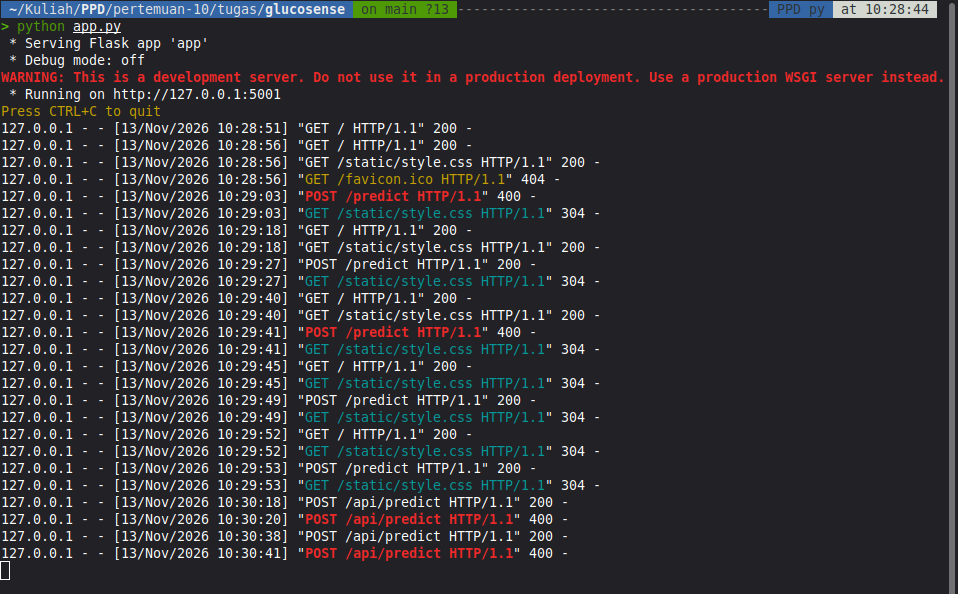
\includegraphics[width=0.88\textwidth]{images/ss-12-jalankan-glucosense.png}
	\caption{Log server GlucoSense selama seluruh pengujian.}
	\label{fig:ss-log-glucosense}
\end{figure}

Log pada Gambar~\ref{fig:ss-log-glucosense} merekam semua pengujian di subbab berikutnya. Baris \texttt{POST /predict} berstatus 400 berasal dari uji validasi form, baris berstatus 200 dari prediksi yang berhasil, dan dua baris terakhir dari uji \texttt{/api/predict} dengan cURL.

\subsection{Pengujian Antarmuka Web}
\begin{figure}[H]
	\centering
	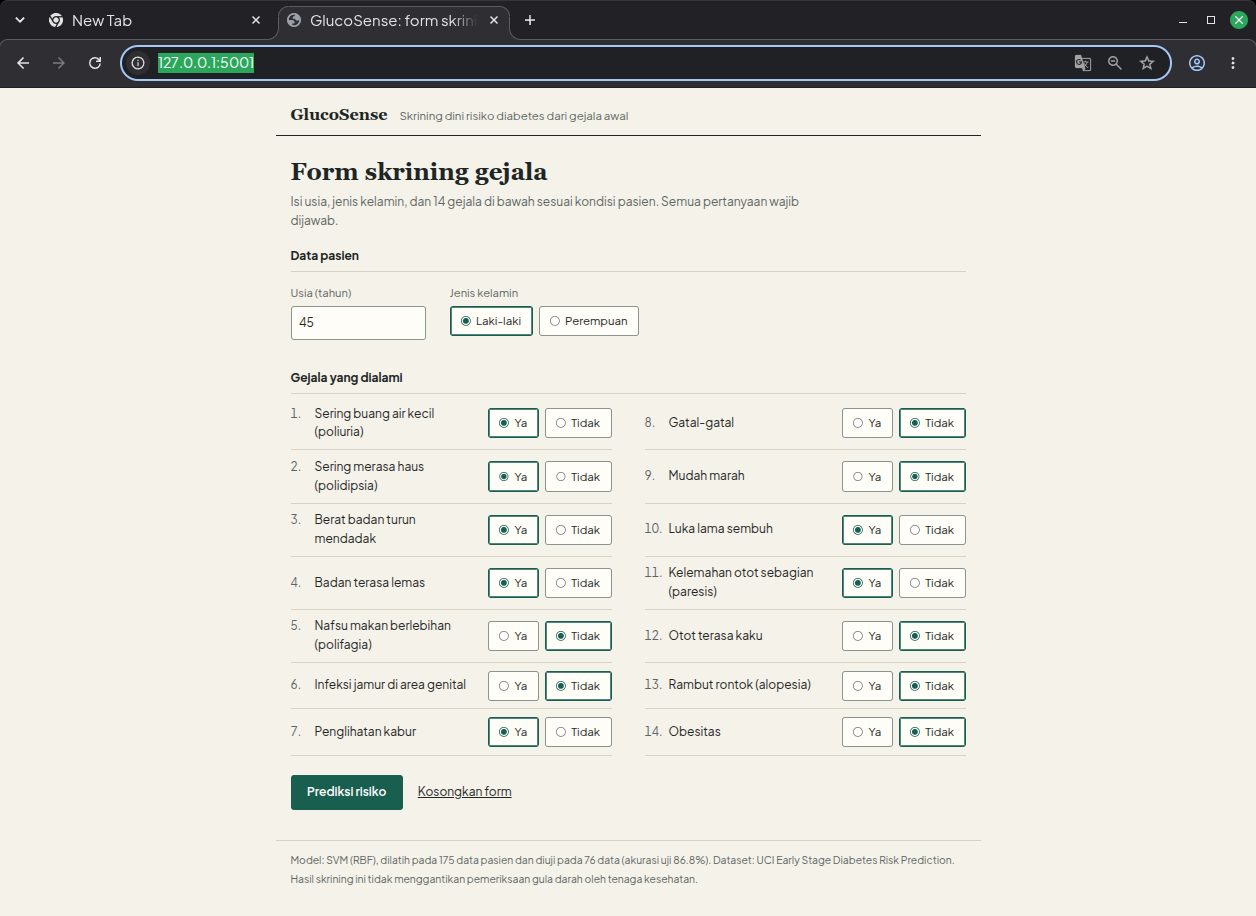
\includegraphics[width=0.9\textwidth]{images/ss-13-form-glucosense.png}
	\caption{Form skrining GlucoSense yang sudah diisi data pasien uji.}
	\label{fig:ss-form-glucosense}
\end{figure}

Form menampilkan gejala dalam bahasa Indonesia dengan pilihan Ya dan Tidak, sehingga pengguna tidak perlu tahu bahwa model sebenarnya menerima angka 1 dan 0. Pasien uji pertama saya isi sebagai laki-laki berusia 45 tahun dengan tujuh gejala, termasuk sering buang air kecil, sering haus, dan berat badan turun mendadak.

\begin{figure}[H]
	\centering
	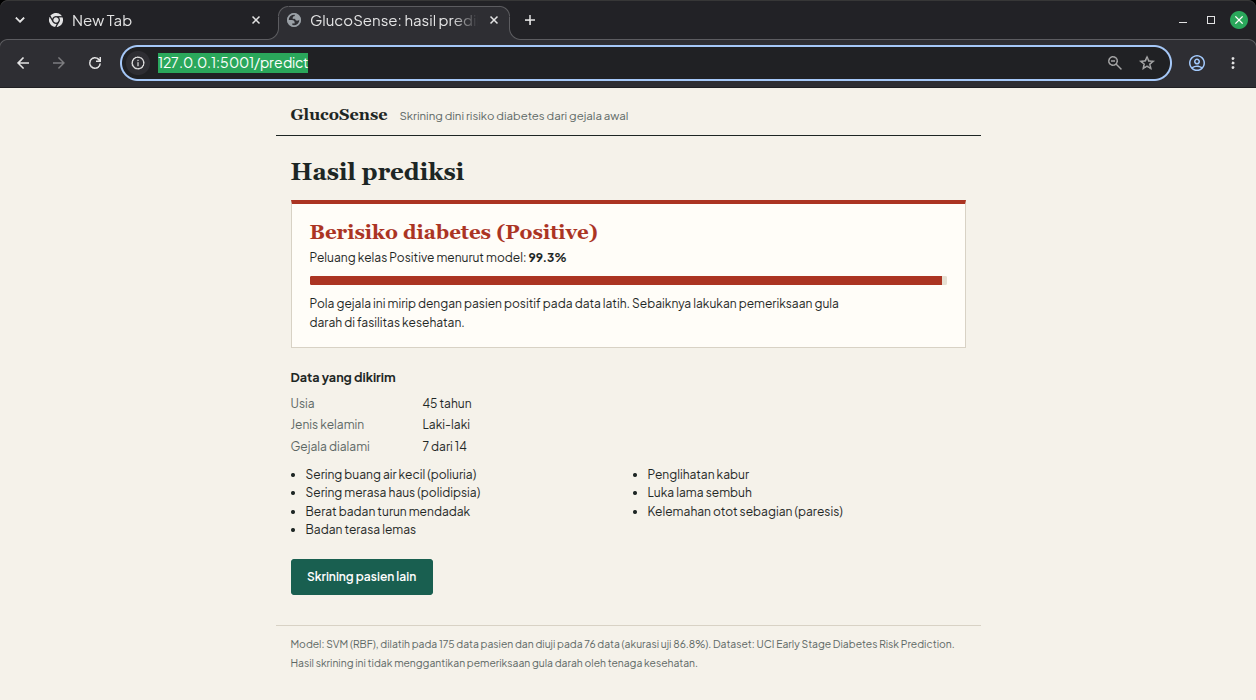
\includegraphics[width=0.9\textwidth]{images/ss-14-hasil-positif.png}
	\caption{Halaman hasil untuk pasien uji pertama: prediksi \textit{Positive}.}
	\label{fig:ss-hasil-positif}
\end{figure}

Model memprediksi pasien ini \textit{Positive} dengan peluang 99,3\%. Halaman hasil juga menampilkan ringkasan data yang dikirim dan daftar gejala yang dijawab Ya, supaya pengguna bisa memeriksa ulang isiannya.

\begin{figure}[H]
	\centering
	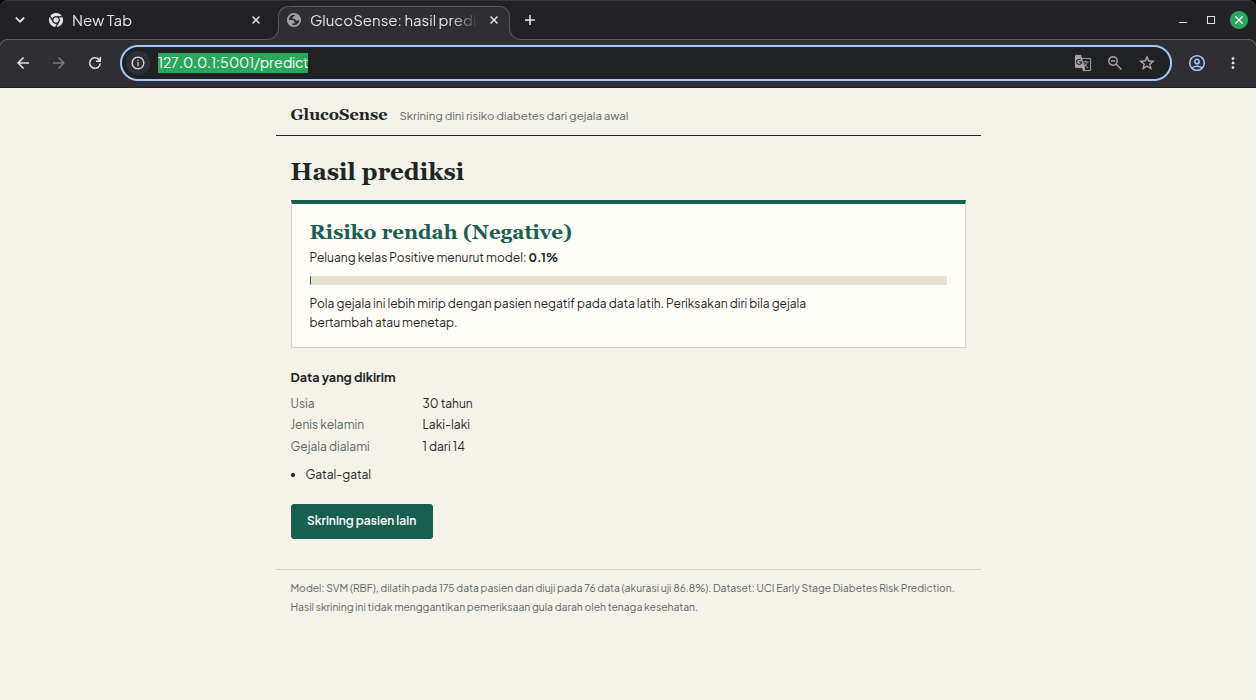
\includegraphics[width=0.9\textwidth]{images/ss-16-hasil-negatif.png}
	\caption{Halaman hasil untuk pasien uji kedua: prediksi \textit{Negative}.}
	\label{fig:ss-hasil-negatif}
\end{figure}

Pasien uji kedua adalah laki-laki berusia 30 tahun yang hanya mengalami gatal-gatal. Model memprediksi \textit{Negative} dengan peluang positif 0,1\%. Kedua hasil ini sejalan dengan temuan kelompok saya bahwa \textit{polyuria} dan \textit{polydipsia} adalah gejala yang paling kuat membedakan kedua kelas. Angka peluang yang sangat dekat dengan 0\% dan 100\% perlu dibaca hati-hati. Model hanya dilatih dengan 175 pasien dari satu rumah sakit, jadi angka itu menggambarkan seberapa mirip isian dengan data latih dan belum tentu mewakili peluang klinis yang sebenarnya.

\begin{figure}[H]
	\centering
	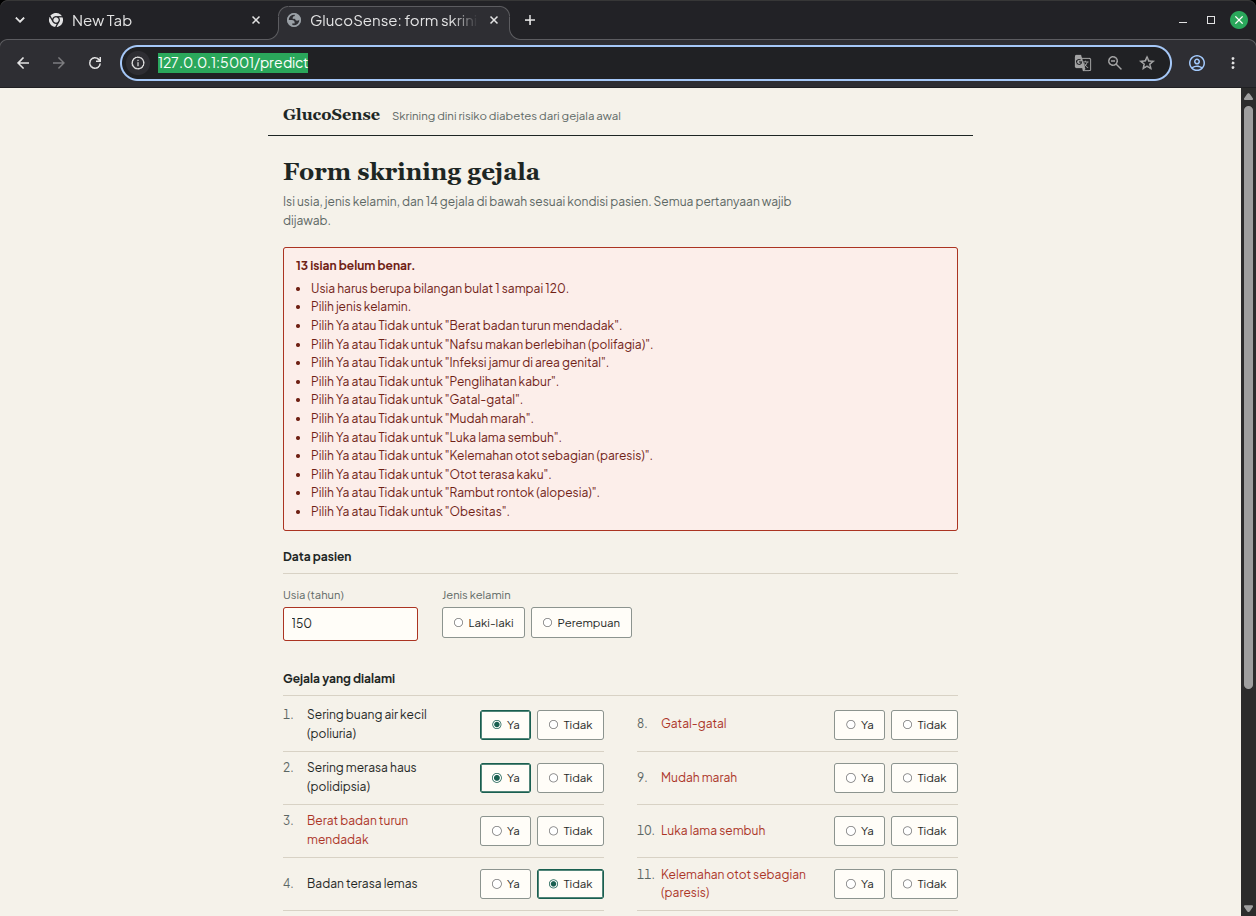
\includegraphics[width=0.9\textwidth]{images/ss-15-validasi-form.png}
	\caption{Pesan validasi saat usia diisi 150 dan sebagian pertanyaan dikosongkan.}
	\label{fig:ss-validasi}
\end{figure}

Untuk menguji validasi, saya mengisi usia 150 dan hanya menjawab tiga gejala. Server menolak kiriman itu dengan status 400 dan menampilkan 13 pesan galat. Tiga jawaban yang sudah diisi tetap terpilih, sehingga pengguna tidak perlu mengulang dari awal. Tanpa validasi ini, isian kosong akan sampai ke model dan menimbulkan galat 500 atau prediksi yang tidak bermakna.

\subsection{Pengujian Endpoint JSON}
\begin{figure}[H]
	\centering
	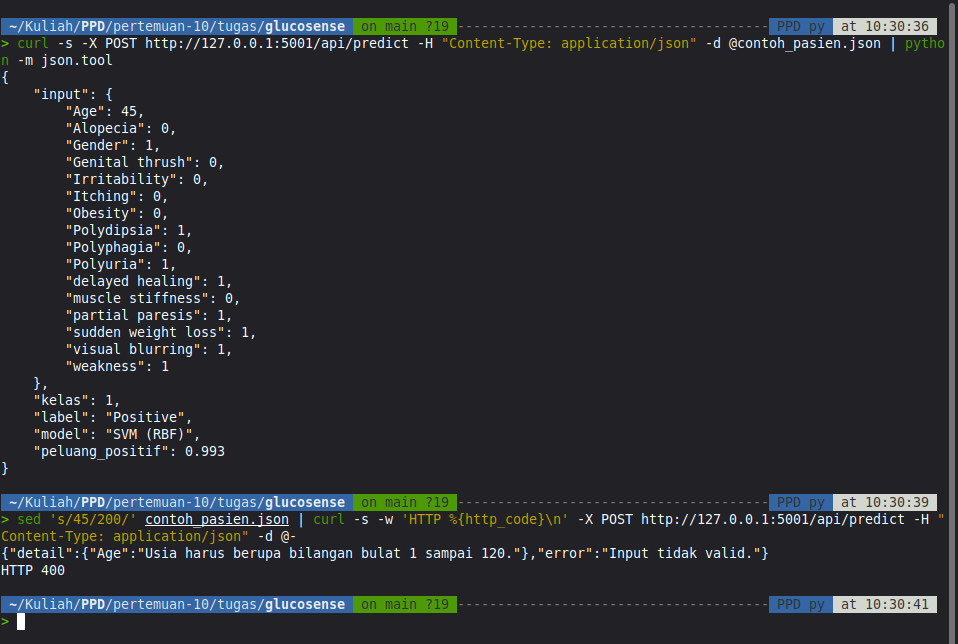
\includegraphics[width=0.88\textwidth]{images/ss-17-uji-api-curl.png}
	\caption{Pengujian \texttt{/api/predict} dengan cURL untuk masukan valid dan tidak valid.}
	\label{fig:ss-api}
\end{figure}

Data pasien uji pertama saya simpan sebagai \texttt{contoh\_pasien.json} lalu saya kirim dengan cURL. Balasannya berupa JSON berisi masukan yang sudah dikodekan menjadi angka, \texttt{kelas} 1, \texttt{label} \textit{Positive}, dan \texttt{peluang\_positif} 0,993. Angka ini sama dengan yang tampil di halaman web untuk pasien yang sama. Pada percobaan kedua, usia saya ganti menjadi 200. Server membalas dengan status 400 dan pesan bahwa usia harus berupa bilangan bulat 1 sampai 120.

\subsection{Analisis}
Dibanding aplikasi modul, ada empat perbedaan pada GlucoSense. Model dimuat sekali saat server mulai. Penskalaan dan model berada dalam satu berkas. Masukan divalidasi sebelum sampai ke model. Selain halaman HTML, tersedia balasan JSON untuk program lain.

Aplikasi ini masih punya beberapa keterbatasan. Server yang dipakai masih server pengembangan Flask dan hanya bisa diakses dari laptop saya sendiri. Supaya bisa dipakai orang lain, aplikasi perlu dijalankan dengan server WSGI seperti Gunicorn dan dipasang di layanan \textit{hosting} \cite{flask-deploy}. Berkas model juga terikat pada scikit-learn 1.9.1, sehingga lingkungan server harus memakai versi yang sama. Dari sisi model, \textit{recall} 0,8654 berarti sekitar satu dari tujuh pasien positif di data uji tidak terdeteksi. Salah satu perbaikan yang bisa dicoba adalah menurunkan ambang peluang di bawah 0,5 agar lebih banyak kasus positif tertangkap, dengan konsekuensi alarm palsu bertambah.

\clearpage

\chapter{Kesimpulan}
Berdasarkan percobaan modul dan tugas yang saya kerjakan pada Pertemuan 10, kesimpulannya adalah sebagai berikut:
\begin{enumerate}[noitemsep, topsep=2pt, parsep=1pt]
	\item \textit{Deployment} dengan skema \textit{client-server} membuat model bisa dipakai lewat peramban tanpa menjalankan ulang kode pelatihan. Pada percobaan modul, model \textit{Decision Tree} penyakit hati berhasil dilayani Flask dan memprediksi \textit{Cirrhosis} untuk isian bawaan form.
	\item Serialisasi dengan \texttt{joblib.dump} menghasilkan berkas model berukuran 5.785 \textit{byte} untuk \textit{Decision Tree} dan 14 KB untuk \texttt{Pipeline} SVM. Keduanya dapat dimuat kembali dengan \texttt{joblib.load} dan langsung dipakai untuk prediksi.
	\item Kode modul yang ditulis tahun 2020 perlu dua penyesuaian di pustaka versi sekarang: label kelas harus diubah menjadi bilangan bulat, dan urutan kolom masukan harus sama dengan urutan saat pelatihan. Karena itu urutan fitur dan versi pustaka sebaiknya disimpan bersama model.
	\item Pada dataset diabetes (251 pasien setelah duplikat dihapus), SVM berkernel RBF terpilih dengan F1 validasi silang 0,9673. Di data uji akurasinya 0,8684 dan F1 0,9000, sedangkan \textit{Random Forest} mencapai akurasi 0,9211. Selisih ini setara 4 dari 76 pasien, jadi belum cukup untuk menyatakan salah satu model lebih unggul.
	\item Aplikasi GlucoSense melayani prediksi lewat form web dan \textit{endpoint} JSON dengan fungsi inferensi yang sama. Pasien uji dengan tujuh gejala diprediksi \textit{Positive} (peluang 99,3\%), pasien dengan satu gejala diprediksi \textit{Negative} (0,1\%), dan masukan yang salah ditolak dengan status 400.
	\item Aplikasi masih berjalan di server pengembangan Flask pada laptop sendiri. Untuk dipakai orang lain, aplikasi perlu server WSGI dan \textit{hosting}, dan \textit{recall} model (0,8654) perlu dinaikkan karena kasus positif yang lolos adalah kesalahan paling merugikan pada alat skrining.
\end{enumerate}

\clearpage

%======================================================================
% DAFTAR PUSTAKA
%======================================================================
\begin{thebibliography}{99}
	\bibitem{repo-kode} H. R. Prasetya, ``Praktikum 10: Model Deployment (Flask),'' GitHub, 2026. [Online]. Tersedia: \url{https://github.com/hafidzrizqullahprasetya/PPD/tree/main/pertemuan-10}.

	\bibitem{breiman1984} L. Breiman, J. H. Friedman, R. A. Olshen, dan C. J. Stone, \textit{Classification and Regression Trees}. Belmont, CA, USA: Wadsworth, 1984.

	\bibitem{cortes1995} C. Cortes dan V. Vapnik, ``Support-vector networks,'' \textit{Machine Learning}, vol. 20, no. 3, hlm. 273 sampai 297, 1995.

	\bibitem{fielding2000} R. T. Fielding, ``Architectural styles and the design of network-based software architectures,'' disertasi doktor, University of California, Irvine, 2000. [Online]. Tersedia: \url{https://ics.uci.edu/~fielding/pubs/dissertation/top.htm}.

	\bibitem{han2022} J. Han, J. Pei, dan H. Tong, \textit{Data Mining: Concepts and Techniques}, edisi ke-4. Cambridge, MA, USA: Morgan Kaufmann, 2022.

	\bibitem{islam2020} M. M. F. Islam, R. Ferdousi, S. Rahman, dan H. Y. Bushra, ``Likelihood prediction of diabetes at early stage using data mining techniques,'' dalam \textit{Computer Vision and Machine Intelligence in Medical Image Analysis}. Singapore: Springer, 2020, hlm. 113 sampai 125.

	\bibitem{joblib-persistence} Joblib developers, ``Persistence,'' Joblib Documentation. [Online]. Tersedia: \url{https://joblib.readthedocs.io/en/stable/persistence.html}.

	\bibitem{uci-hcv} R. Lichtinghagen, F. Klawonn, dan G. Hoffmann, ``HCV data,'' UCI Machine Learning Repository, 2020. [Online]. Tersedia: \url{https://doi.org/10.24432/C5D612}.

	\bibitem{flask-quickstart} Pallets, ``Quickstart,'' Flask Documentation. [Online]. Tersedia: \url{https://flask.palletsprojects.com/en/stable/quickstart/}.

	\bibitem{flask-deploy} Pallets, ``Deploying to production,'' Flask Documentation. [Online]. Tersedia: \url{https://flask.palletsprojects.com/en/stable/deploying/}.

	\bibitem{sklearn2011} F. Pedregosa \textit{et al.}, ``Scikit-learn: Machine learning in Python,'' \textit{Journal of Machine Learning Research}, vol. 12, hlm. 2825 sampai 2830, 2011.

	\bibitem{platt1999} J. C. Platt, ``Probabilistic outputs for support vector machines and comparisons to regularized likelihood methods,'' dalam \textit{Advances in Large Margin Classifiers}. Cambridge, MA, USA: MIT Press, 1999, hlm. 61 sampai 74.

	\bibitem{python-pickle} Python Software Foundation, ``pickle: Python object serialization,'' Python 3 Documentation. [Online]. Tersedia: \url{https://docs.python.org/3/library/pickle.html}.

	\bibitem{sklearn-persistence} Scikit-learn developers, ``Model persistence,'' Scikit-learn Documentation. [Online]. Tersedia: \url{https://scikit-learn.org/stable/model_persistence.html}.

	\bibitem{sklearn-calibration} Scikit-learn developers, ``Probability calibration,'' Scikit-learn Documentation. [Online]. Tersedia: \url{https://scikit-learn.org/stable/modules/calibration.html}.

	\bibitem{uci-diabetes} UCI Machine Learning Repository, ``Early stage diabetes risk prediction dataset,'' 2020. [Online]. Tersedia: \url{https://doi.org/10.24432/C5VG8H}.
\end{thebibliography}

\end{document}
